%%%%%%%%%%%%%%%%%%%%%%%%%%%%%%%%%%%%%%%%%
% Beamer Presentation
% LaTeX Template
% Version 1.0 (10/11/12)
%
% This template has been downloaded from:
% http://www.LaTeXTemplates.com
%
% License:
% CC BY-NC-SA 3.0 (http://creativecommons.org/licenses/by-nc-sa/3.0/)
%
%%%%%%%%%%%%%%%%%%%%%%%%%%%%%%%%%%%%%%%%%

%----------------------------------------------------------------------------------------
%	PACKAGES AND THEMES
%----------------------------------------------------------------------------------------

\documentclass[usenames,dvipsnames]{beamer}

\mode<presentation> {

% The Beamer class comes with a number of default slide themes
% which change the colors and layouts of slides. Below this is a list
% of all the themes, uncomment each in turn to see what they look like.

%\usetheme{default}
% \usetheme{AnnArbor}
%\usetheme{Antibes}
%\usetheme{Bergen}
% \usetheme{Berkeley}
% \usetheme{Berlin}
%\usetheme{Boadilla}
%\usetheme{CambridgeUS}
% \usetheme{Copenhagen}
\usetheme{Darmstadt}
% \usetheme{Dresden}
% \usetheme{Frankfurt}
% \usetheme{Goettingen}
%\usetheme{Hannover}
%\usetheme{Ilmenau}
%\usetheme{JuanLesPins}
%\usetheme{Luebeck}
% \usetheme{Madrid}
% \usetheme{Malmoe}
%\usetheme{Marburg}
% \usetheme{Montpellier}
% \usetheme{PaloAlto}
% \usetheme{Pittsburgh}
%\usetheme{Rochester}
% \usetheme{Singapore}
%\usetheme{Szeged}
%\usetheme{Warsaw}

% As well as themes, the Beamer class has a number of color themes
% for any slide theme. Uncomment each of these in turn to see how it
% changes the colors of your current slide theme.

% \usecolortheme{albatross}
%\usecolortheme{beaver}
%\usecolortheme{beetle}
%\usecolortheme{crane}
%\usecolortheme{dolphin}
%\usecolortheme{dove}
%\usecolortheme{fly}
\usecolortheme{lily}
%\usecolortheme{orchid}
%\usecolortheme{rose}
%\usecolortheme{seagull}
%\usecolortheme{seahorse}
%\usecolortheme{whale}
%\usecolortheme{wolverine}

%\setbeamertemplate{footline} % To remove the footer line in all slides uncomment this line
%\setbeamertemplate{footline}[page number] % To replace the footer line in all slides with a simple slide count uncomment this line

%\setbeamertemplate{navigation symbols}{} % To remove the navigation symbols from the bottom of all slides uncomment this line
}

% % -------------------------------------------
% % Songkai added, feel free to delete --------
% \AtBeginSection[]{
%   \begin{frame}
%   \vfill
%   \centering
%   \begin{beamercolorbox}[sep=8pt,center,shadow=false,rounded=true]{title}
%     \usebeamerfont{title}\insertsectionhead\par%
%   \end{beamercolorbox}
%   \vfill
%   \end{frame}
% }
% % Songkai added, feel free to delete --------
% % -------------------------------------------

\usepackage{graphicx} % Allows including images
\usepackage{booktabs} % Allows the use of \toprule, \midrule and \bottomrule in tables
\usepackage{natbib}
\usepackage{xcolor}
\usepackage{amsmath, amssymb, graphicx, url}
\usepackage[ruled]{algorithm2e}
\usepackage{commath}
\usefonttheme[onlymath]{serif}

% \usepackage{amsmath}
% \usepackage{amssymb}
%\usepackage[a4paper, margin=0.8in]{geometry}
\usepackage{parskip}
% \usepackage{graphicx}

% \usepackage{natbib}
% \usepackage[colorlinks=true, linkcolor={blue}]{hyperref}

\hypersetup{pdfauthor={Name},colorlinks=true, linkcolor={white}, citecolor={teal}}

\usepackage{tabularx}
\usepackage{array}
\usepackage{makecell}
\usepackage{mathtools}
\usepackage{bm,upgreek}
\usepackage{bbm}
\usepackage{dsfont}
\usepackage{textpos}
% \usepackage{eso-pic}

\def\E{\mathbf{E}}
\def\PP{\mathbf{P}}
\def\Reals{\mathbb{R}}
\def\Naturals{\mathbb{N}}
\def\argmin{\operatornamewithlimits{arg\,min}}
\def\deq{:=}
\def\wh#1{\widehat{#1}}
\def\bd#1{\mathbf{#1}}
\def\bx{\bd{x}}
\def\by{\bd{y}}
\def\bZ{\bd{Z}}
\def\bB{\bd{B}}
\def\bV{\bd{V}}
\def\tO{{\tilde{\cO}}}
\def\tOm{\tilde{\Omega}}
\def\barw{\overline{w}}
\def\d{{\mathrm d}}
\def\ave#1{\langle #1 \rangle}
\def\Ave#1{\left\langle #1 \right\rangle}
\def\eps{\varepsilon}
\def\tr{\mathrm{Tr}}


\def\HS{\mathbb{H}}
\def\reals{\mathbb{R}}
\def\ths{\theta^*}
\def\thh{\hat{\theta}}
\def\lbr{\left[}
\def\rbr{\right]}
\def\lc{\left(}
\def\rc{\right)}


    \def\ddefloop#1{\ifx\ddefloop#1\else\ddef{#1}\expandafter\ddefloop\fi}
    % \cA, \cB, ...
    \def\ddef#1{\expandafter\def\csname c#1\endcsname{\ensuremath{\mathcal{#1}}}}
    \ddefloop ABCDEFGHIJKLMNOPQRSTUVWXYZ\ddefloop
    \def\argmin{\operatornamewithlimits{arg\,min}}
    \def\E{\mathbf{E}}
    \def\bx{\bd{x}}
	\def\by{\bd{y}}
    \def\bZ{\bd{Z}}

\newcommand{\propnumber}{} % initialize
\newtheorem*{prop}{Proposition \propnumber}
\newenvironment{propc}[1]
  {\renewcommand{\propnumber}{#1}%
   \begin{shaded}\begin{prop}}
  {\end{prop}\end{shaded}}

\newcommand{\crlrnumber}{} % initialize
%\newtheorem*{corollary}{Corollary \crlrnumber}
\newenvironment{corollaryc}[1]
  {\renewcommand{\crlrnumber}{#1}%
   \begin{shaded}\begin{corollary}}
  {\end{corollary}\end{shaded}}

\theoremstyle{definition}
% \newtheorem{definition}




% \setbeamertemplate{headline}{% 
%     \leavevmode%
%     \hbox{%
%         \begin{beamercolorbox}[wd=.4\paperwidth,ht=2.25ex,dp=1ex,right]{section in head/foot}%
%             \usebeamerfont{section in head/foot}\insertshorttitle\hspace*{2ex}
%         \end{beamercolorbox}%
%         \begin{beamercolorbox}[wd=.6\paperwidth,ht=2.25ex,dp=1ex,left]{subsection in head/foot}%
%             \usebeamerfont{section in head/foot}
\includegraphics[height=2ex,keepaspectratio]{Slides/Block_M-Hex.png}\hspace*{2ex}\insertsectionhead
%         \end{beamercolorbox}%
%     }
% }

% \addtobeamertemplate{headline}{}{%
% \begin{textblock*}{100mm}(.85\textwidth,-1cm)
% \Huge\textcolor{white}{\textbf{\TeX}}
% \end{textblock*}}



%----------------------------------------------------------------------------------------
%	TITLE PAGE
%----------------------------------------------------------------------------------------

%%%% TRY WITH TEXTPOS
% \newcommand{\imgblock}{\begin{textblock*}{5cm}(10.5cm,-1.2cm) % {block width} (coords)
%         
\includegraphics[width=1cm]{Slides/Block_M-Hex.png} % loading the image
%     \end{textblock*}
%     }

% \addtobeamertemplate{background}{\imgblock}{}



% \setbeamertemplate{headline}{\hfill
\includegraphics[width=1.5cm]{Slides/Block_M-Hex.png}\hspace{0.2cm}\vspace{-1cm}}

% \logo{
\includegraphics[height=1cm]{Slides/Block_M-Hex.png}}

\addtobeamertemplate{frametitle}{}{%
    \begin{textblock*}{5cm}(10.5cm, -0.8cm)
        
\includegraphics[width=0.9cm]{Slides/Block_M-Hex.png} % your logo file here
    \end{textblock*}
}

\usepackage{xcolor}
\definecolor{mycolor}{cmyk}{100, 60, 0, 60}


% \setbeamertemplate{footline}[text line]{%
%   \parbox{\linewidth}{\vspace*{-8pt}some text\hfill\insertshortauthor\hfill\insertshorttitle\hfill\insertshortinstitute}}
% \setbeamertemplate{navigation symbols}{}

\setbeamercolor{frametitle}{bg=mycolor}

\title[Journal Club]{Reading Group: Time Series CP} % The short title appears at the bottom of every slide, the full title is only on the title page

\author[Aniket Jivani]{Aniket Jivani}
\institute[U-M]{University of Michigan}

\date{\today}

\begin{document}

\begin{frame}
\titlepage % Print the title page as the first slide
\end{frame}



\begin{frame}
 \frametitle{Overview} % Table of contents slide, comment this block out to remove it
 \tableofcontents % Throughout your presentation, if you choose to use \section{} and \subsection{} commands, these will automatically be printed on this slide as an overview of your presentation
\end{frame}

\section{Introduction}
\begin{frame}{Key Papers}
    \begin{itemize}
        \item Conformal Prediction for Time Series \cite{xu_conformal_2023}

        \item Sequential Predictive Conformal Inference for Time Series \cite{pmlr-v202-xu23r}
    \end{itemize}
\end{frame}

\begin{frame}{Motivation}
    \begin{itemize}
        \item \textbf{Conformal Prediction} - coverage guarantee with arbitrary prediction algorithms, simple recipe to apply to neural networks by calculation of non-conformity scores on held-out data

        \item However, we cannot extend these methods to time series easily - not exchangeable i.e. no significance of time dimension is a bad assumption

        \item Existing methods (I think they only talk about non-BNN approaches :-) either strong parametric distributional assumptions (autoregressive models? \url{https://otexts.com/fpp2/non-seasonal-arima.html}) OR restricted to specific model architectures of deep neural networks - \cite{wen_multi-horizon_2017} 
    \end{itemize}
\end{frame}

\begin{frame}{Backup - multi-step quantiles from RNNs}
    \begin{itemize}
        \item Return full conditional distributions $p(y_{t + k} | y_{1:t})$
        
    \end{itemize}
\end{frame}

\begin{frame}{Backup - Pinball loss}
\begin{columns}
\begin{column}{0.48\textwidth}
    \begin{figure}
        \centering
        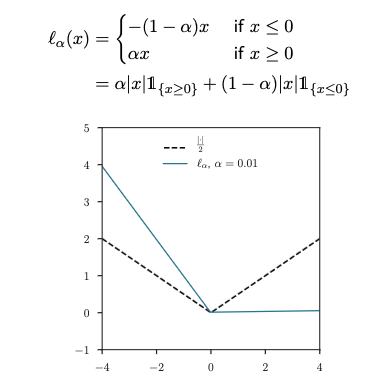
\includegraphics[scale=0.35]{Slides/pinball.png}
        \caption{Pinball loss}
        \label{fig:pblloss}
    \end{figure}
\end{column}
\begin{column}{0.56\textwidth}  %%<--- here
    \begin{itemize}
        \item See: \href{https://josephsalmon.eu/enseignement/UW/STAT593/QuantileRegression.pdf}{QR Notes}
        \item Define $$\check{\mu}\in\operatorname{arg}\min_{\mu\in\mathbb{R}}\mathbb{E}_{F}\big(\ell_{\alpha}(X-\mu)\big)$$

        when $\ell_{\alpha}(x):=\alpha|x|\mathbbm{1}_{\{x\geq0\}}+(1-\alpha)|x|\mathbbm{1}_{\{x\leq0\}}$
        
        % \text{when}&\ell_{\alpha}(x):=\alpha|x|\mathds{1}_{\{x\geq0\}}+(1-\alpha)|x|\mathds{1}_{\{x\leq0\}}\text{then}\end{aligned}
        \item then $\check{\mu} = F^{-1}(\alpha) = q_{X}(\alpha)$ is the $\alpha$--quantile of distribution $F$
        \item In regression setting - $\alpha$--th quantile is defined as:
        $$\hat{\beta}^{\alpha}\in\arg\min_{\beta\in\mathbb{R}^{p}}\sum_{i=1}^{n}\ell_{\alpha}(y_{i}-\langle x_{i},\beta\rangle)$$
    \end{itemize}
\end{column}
\end{columns}
\end{frame}

\section{Time Series}
\begin{frame}{Proposed Method Claims}
    \begin{itemize}
        \item General framework for time-series without exchangeability, upper bounds on conditional and marginal coverage

        \item Procedure avoids expensive model retraining on account of bootstrap-like step prior to LOO predictors

        \item Maintains target coverage and has smaller intervals compared to competing methods, robust to missing data etc.
    \end{itemize}
\end{frame}

\begin{frame}{Notation}
    
\end{frame}


\begin{frame}{Pseudocode}
    
\end{frame}

\begin{frame}{Assumptions}
    \begin{enumerate}
        \item \textcolor{violet}{\emph{Errors are short-term i.i.d}}

        \item \textcolor{violet}{\emph{Asymptotic guarantee for estimator convergence to true value}}
    \end{enumerate}

    In short, coverage guarantees won't hold for poor choice of model $+$ highly non-stationary data 
\end{frame}

\begin{frame}{Coverage Properties and Proof Sketch}

\end{frame}

\begin{frame}{Coverage Properties and Proof Sketch}

\end{frame}
\section{Results}

\begin{frame}{Example 1}
    
\end{frame}

\begin{frame}{Example 2}
    
\end{frame}

\begin{frame}{Construct failure case?}
    
\end{frame}

\section{Wrap-up}
\begin{frame}{Key takeaways}
    
\end{frame}

\begin{frame}{Limitations}
    
\end{frame}

\begin{frame}{References}
\bibliographystyle{chicago}

%\bibliographystyle{IEEEtran}
\bibliography{myReference}
    
\end{frame}


\begin{frame}{}
\begin{center}
    \Large{Thank you!}
\end{center}
    
\end{frame}


\end{document}